\documentclass[14pt]{extbook}
\usepackage{multicol, enumerate, enumitem, hyperref, color, soul, setspace, parskip, fancyhdr} %General Packages
\usepackage{amssymb, amsthm, amsmath, latexsym, units, mathtools} %Math Packages
\everymath{\displaystyle} %All math in Display Style
% Packages with additional options
\usepackage[headsep=0.5cm,headheight=12pt, left=1 in,right= 1 in,top= 1 in,bottom= 1 in]{geometry}
\usepackage[usenames,dvipsnames]{xcolor}
\usepackage{dashrule}  % Package to use the command below to create lines between items
\newcommand{\litem}[1]{\item#1\hspace*{-1cm}\rule{\textwidth}{0.4pt}}
\pagestyle{fancy}
\lhead{Progress Quiz 7}
\chead{}
\rhead{Version A}
\lfoot{4173-5738}
\cfoot{}
\rfoot{Spring 2021}
\begin{document}

\begin{enumerate}
\litem{
Solve the radical equation below. Then, choose the interval(s) that the solution(s) belongs to.\[ \sqrt{20 x^2 + 21} - \sqrt{-43 x} = 0 \]\begin{enumerate}[label=\Alph*.]
\item \( x \in [-1.1,-0.29] \)
\item \( x_1 \in [-2.13, -0.84] \text{ and } x_2 \in [-1.75,0.25] \)
\item \( x \in [-2.13,-0.84] \)
\item \( x_1 \in [-0.61, 1.35] \text{ and } x_2 \in [-0.6,2.4] \)
\item \( \text{All solutions lead to invalid or complex values in the equation.} \)

\end{enumerate} }
\litem{
Choose the equation of the function graphed below.
\begin{center}
    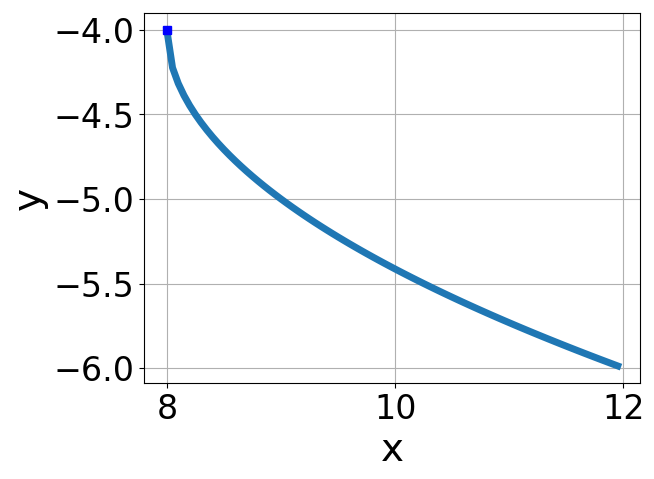
\includegraphics[width=0.5\textwidth]{../Figures/radicalGraphToEquationA.png}
\end{center}
\begin{enumerate}[label=\Alph*.]
\item \( f(x) = - \sqrt[3]{x + 10} - 6 \)
\item \( f(x) = - \sqrt[3]{x - 10} - 6 \)
\item \( f(x) = \sqrt[3]{x + 10} - 6 \)
\item \( f(x) = \sqrt[3]{x - 10} - 6 \)
\item \( \text{None of the above} \)

\end{enumerate} }
\litem{
Solve the radical equation below. Then, choose the interval(s) that the solution(s) belongs to.\[ \sqrt{-40 x^2 - 42} - \sqrt{86 x} = 0 \]\begin{enumerate}[label=\Alph*.]
\item \( x \in [-1.24,-0.65] \)
\item \( \text{All solutions lead to invalid or complex values in the equation.} \)
\item \( x_1 \in [1.05, 1.72] \text{ and } x_2 \in [0.2,1.8] \)
\item \( x_1 \in [-2.24, -1.3] \text{ and } x_2 \in [-2.8,-0.5] \)
\item \( x \in [-2.24,-1.3] \)

\end{enumerate} }
\litem{
Choose the graph of the equation below.\[ f(x) = - \sqrt[3]{x - 6} + 5 \]\begin{enumerate}[label=\Alph*.]
\begin{multicols}{2}\item 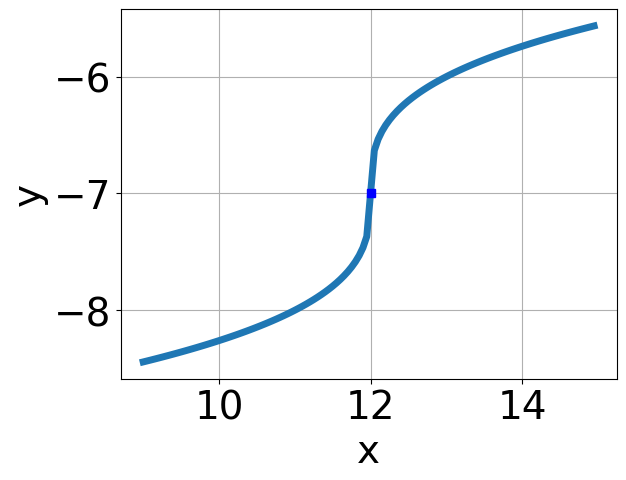
\includegraphics[width = 0.3\textwidth]{../Figures/radicalEquationToGraphAA.png}\item 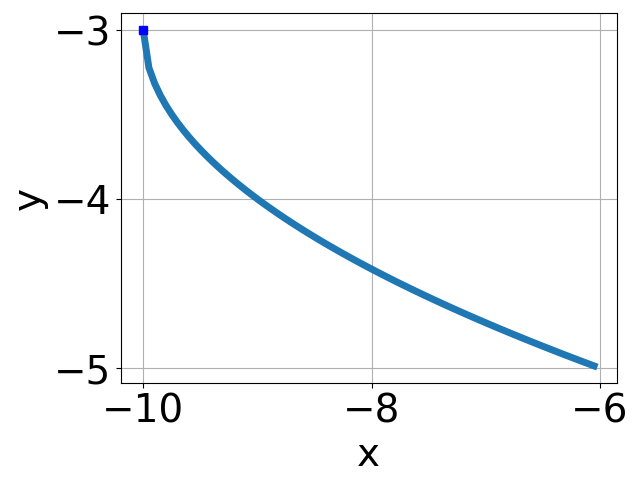
\includegraphics[width = 0.3\textwidth]{../Figures/radicalEquationToGraphBA.png}\item 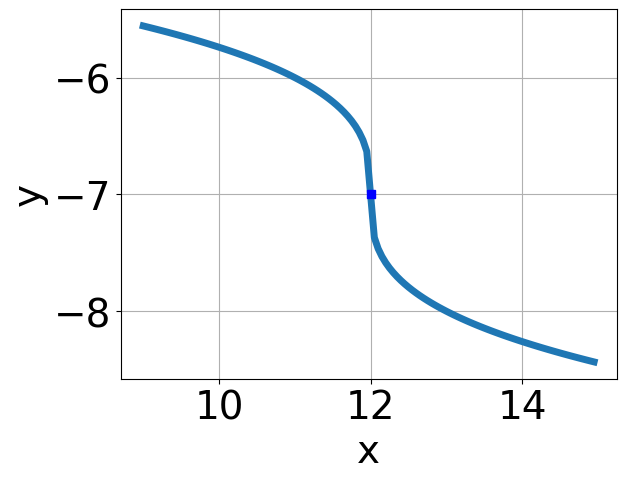
\includegraphics[width = 0.3\textwidth]{../Figures/radicalEquationToGraphCA.png}\item 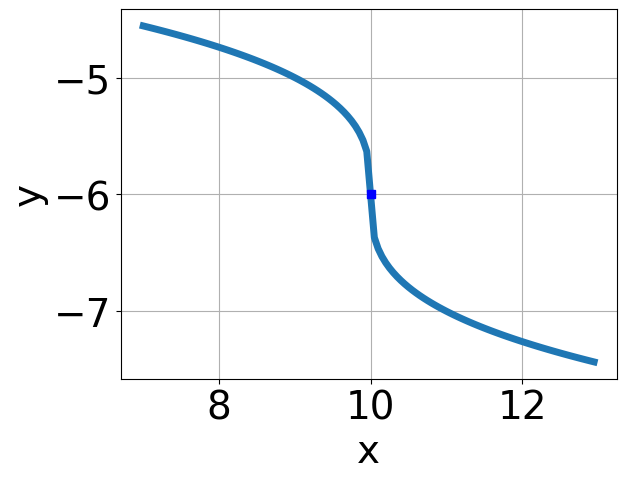
\includegraphics[width = 0.3\textwidth]{../Figures/radicalEquationToGraphDA.png}\end{multicols}\item None of the above.
\end{enumerate} }
\litem{
Solve the radical equation below. Then, choose the interval(s) that the solution(s) belongs to.\[ \sqrt{3 x - 9} - \sqrt{-9 x - 5} = 0 \]\begin{enumerate}[label=\Alph*.]
\item \( \text{All solutions lead to invalid or complex values in the equation.} \)
\item \( x_1 \in [-0.5, 0.5] \text{ and } x_2 \in [3,8] \)
\item \( x \in [0.7,1.6] \)
\item \( x \in [-0.5,0.5] \)
\item \( x_1 \in [-1.8, -0.1] \text{ and } x_2 \in [3,8] \)

\end{enumerate} }
\litem{
Choose the graph of the equation below.\[ f(x) = \sqrt{x - 8} + 7 \]\begin{enumerate}[label=\Alph*.]
\begin{multicols}{2}\item 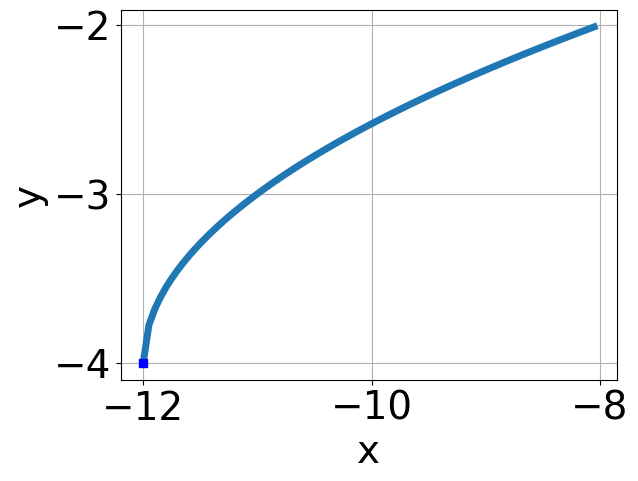
\includegraphics[width = 0.3\textwidth]{../Figures/radicalEquationToGraphCopyAA.png}\item 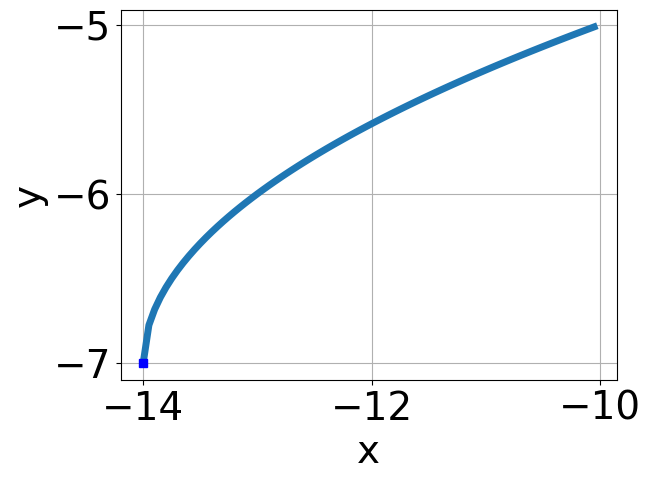
\includegraphics[width = 0.3\textwidth]{../Figures/radicalEquationToGraphCopyBA.png}\item 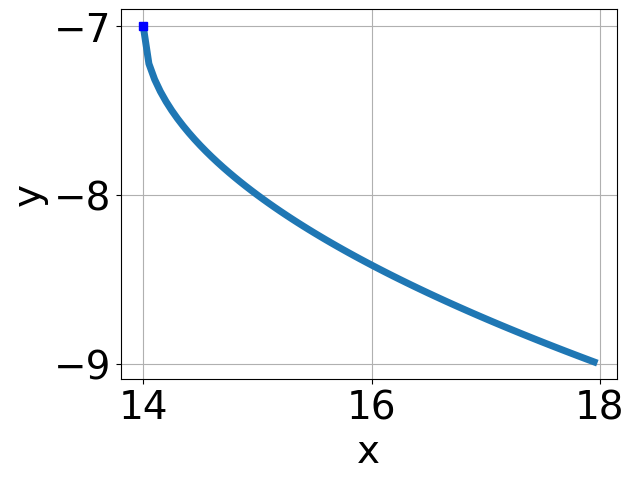
\includegraphics[width = 0.3\textwidth]{../Figures/radicalEquationToGraphCopyCA.png}\item 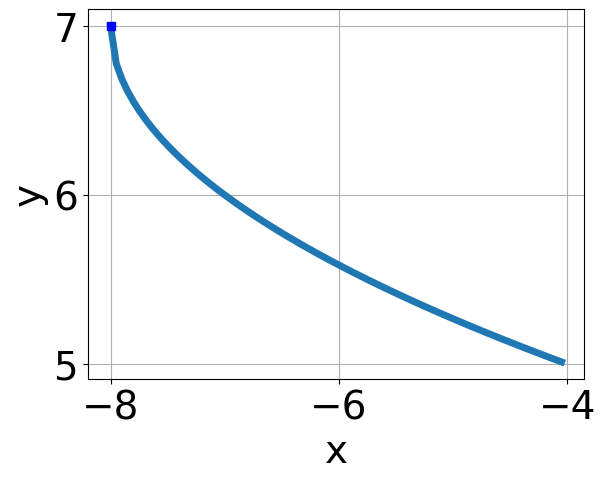
\includegraphics[width = 0.3\textwidth]{../Figures/radicalEquationToGraphCopyDA.png}\end{multicols}\item None of the above.
\end{enumerate} }
\litem{
What is the domain of the function below?\[ f(x) = \sqrt[3]{-4 x - 6} \]\begin{enumerate}[label=\Alph*.]
\item \( \text{The domain is } [a, \infty), \text{   where } a \in [-1.62, -1.35] \)
\item \( \text{The domain is } (-\infty, a], \text{   where } a \in [-1.47, 1.22] \)
\item \( \text{The domain is } (-\infty, a], \text{   where } a \in [-2.77, -1.25] \)
\item \( (-\infty, \infty) \)
\item \( \text{The domain is } [a, \infty), \text{   where } a \in [-1.42, -0.32] \)

\end{enumerate} }
\litem{
What is the domain of the function below?\[ f(x) = \sqrt[3]{-5 x - 6} \]\begin{enumerate}[label=\Alph*.]
\item \( \text{The domain is } (-\infty, a], \text{   where } a \in [-1.03, -0.56] \)
\item \( (-\infty, \infty) \)
\item \( \text{The domain is } [a, \infty), \text{   where } a \in [-1.78, -1.09] \)
\item \( \text{The domain is } (-\infty, a], \text{   where } a \in [-1.85, -1.04] \)
\item \( \text{The domain is } [a, \infty), \text{   where } a \in [-1.11, -0.33] \)

\end{enumerate} }
\litem{
Solve the radical equation below. Then, choose the interval(s) that the solution(s) belongs to.\[ \sqrt{5 x + 4} - \sqrt{-5 x - 7} = 0 \]\begin{enumerate}[label=\Alph*.]
\item \( x_1 \in [-1.88, -1.13] \text{ and } x_2 \in [-1.8,4.2] \)
\item \( x \in [-1.27,-0.29] \)
\item \( x_1 \in [-1.27, -0.29] \text{ and } x_2 \in [-1.8,4.2] \)
\item \( x \in [-0.12,1.21] \)
\item \( \text{All solutions lead to invalid or complex values in the equation.} \)

\end{enumerate} }
\litem{
Choose the equation of the function graphed below.
\begin{center}
    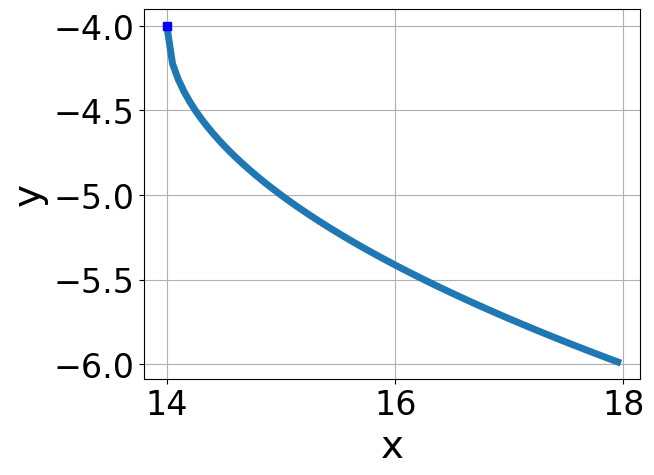
\includegraphics[width=0.5\textwidth]{../Figures/radicalGraphToEquationCopyA.png}
\end{center}
\begin{enumerate}[label=\Alph*.]
\item \( f(x) = - \sqrt[3]{x - 8} - 7 \)
\item \( f(x) = - \sqrt[3]{x + 8} - 7 \)
\item \( f(x) = \sqrt[3]{x - 8} - 7 \)
\item \( f(x) = \sqrt[3]{x + 8} - 7 \)
\item \( \text{None of the above} \)

\end{enumerate} }
\end{enumerate}

\end{document}